\documentclass{beamer}
\mode<presentation> {
    \usetheme{Copenhagen} \usecolortheme{whale}
    }
\usepackage{graphicx}
\usepackage{multicol}
\setbeamersize{text margin left=3mm,text margin right=5mm}

\graphicspath{{Images/}}

\title[Assignments 4]{MRAC e I\&I}
\author{Lorenzo Rossi Matricola: 0301285}
\begin{document}
\begin{frame}
	\titlepage{}
\end{frame}
\begin{frame}
	\begin{columns}[t]
		\begin{column}{.5\textwidth}
			\tableofcontents[sections={1-3}] % chktex 8
		\end{column}
		\hspace{-1cm}
		\begin{column}{.5\textwidth}
			\tableofcontents[sections={4-5}] % chktex 8
		\end{column}
	\end{columns}
\end{frame}
\begin{frame}
	\frametitle{Assignment 4}
	\section{Introduzione}
	Considerato il sistema:\begin{equation*}
		\dot{x}=ax+u\quad a\text{ non noto}
	\end{equation*}
	Effettua le simulazioni con \(a=1 \text{e} a_{m}=1\) e implementa un controllore adattativo MRAC e I\&I per risolvere il problema di regolazione adattativa. Inoltre, confronta le performance dei due controllori in presenza di rumore additivo \begin{equation*}
		x+d\quad d(t) = 0.1 \sin{\frac{1}{5}}
	\end{equation*}
	Infine, contronta le performance nel caso in cui il parametro \(a\) del sistema è del tipo:
	\begin{equation*}
		a=1+\frac{1}{10}\sin{10t}\quad a=1+10\sin{\frac{t}{10}}
	\end{equation*}
\end{frame}
\begin{frame}
	\frametitle{Modello teorico}
	\section{Modello teorico}
	\begin{itemize}
		\item \textbf{Modello di riferimento:}\(\dot{x_{m}}=-a_{m}x_{m}\);
		\item \textbf{Sistema:}\(\dot{x}=ax+u\);
		\item \textbf{Controllore adattativo I\&I:}\begin{itemize}
			      \item \emph{\(\beta\) quadratic:}\(\dot{x}=-a_{m}x-xz,\dot{z}=-x^{2}z,\dot{\hat{a}}=a_{m}x^{2},a_{est}=\hat{a}+\frac{x^{2}}{2}\)
			      \item \emph{\(\beta\) logarithmic:}\(\dot{x}=-a_{m}x-xz,\dot{z}=-\frac{a_{m}x^{2}}{1+x^{2}},\dot{\hat{a}}=a_{m}\frac{x^{2}}{1+x^{2}},a_{est}=\hat{a}+\frac{1}{2}\log{(1+x^{2})}\)
		      \end{itemize}
		\item \textbf{Controllore MRAC:}\(\dot{\tilde{k}}=\gamma \varepsilon_{1}x,u=-\tilde{k}x,\varepsilon_{1}=x-\hat{x}\)
	\end{itemize}
\end{frame}
\begin{frame}
	\frametitle{Simulink - 1}% chktex 8
	\section{Implementazione Simulink}
	\subsection{Reference Model}
	\begin{minipage}[t]{0.45\textwidth}
		\begin{itemize}

			\item \textbf{Reference Model:}
			      \begin{figure}
				      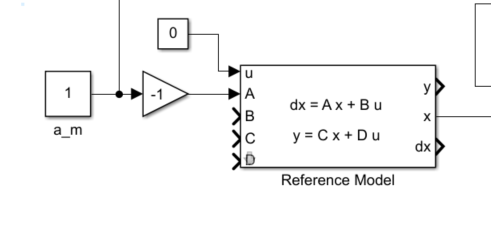
\includegraphics[scale=0.4]{2022-05-19-18-26-28.png}% chktex 8
			      \end{figure}
		\end{itemize}
	\end{minipage}
	\begin{minipage}[t]{0.45\textwidth}
		\begin{itemize}
			\item \textbf{Sistema:}
			      \begin{figure}
				      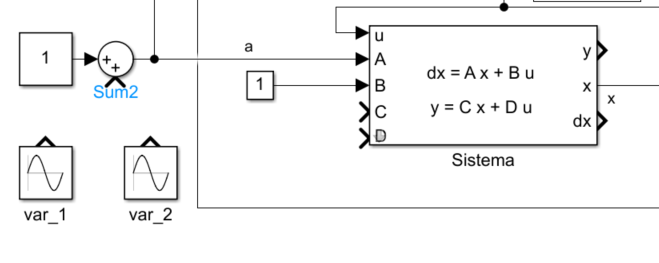
\includegraphics[scale=0.3]{2022-05-19-18-30-54.png}% chktex 8
			      \end{figure}
		\end{itemize}
	\end{minipage}
\end{frame}
\begin{frame}
	\frametitle{Simulink-2}% chktex 8
	\subsection{Controllo Adattativo I\&I}
	\subsubsection{\(\beta\) quadratic}
	\begin{itemize}
		\item \textbf{I\&I \(\beta\) quadratic:}
		\begin{figure}
			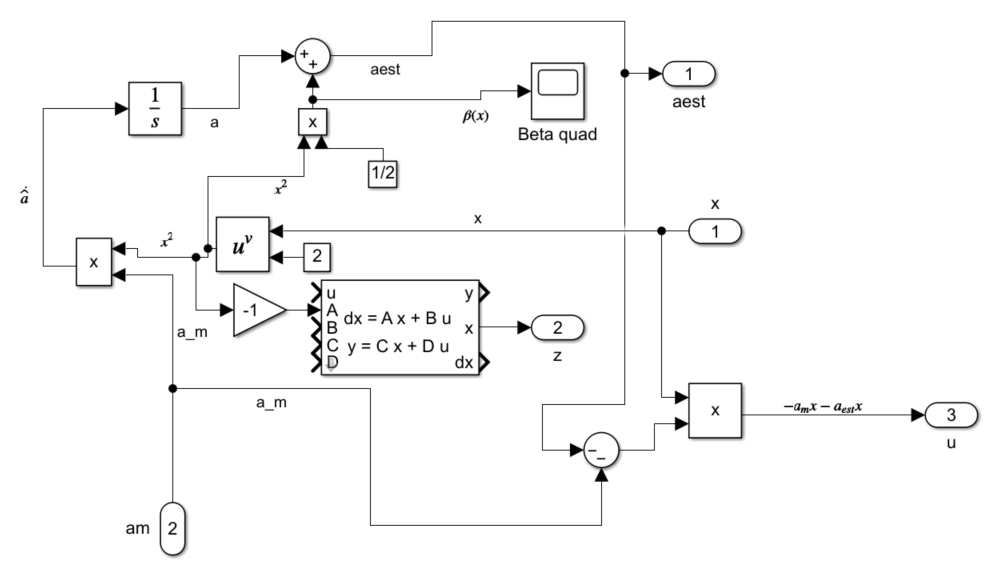
\includegraphics[scale=0.3]{2022-05-19-18-34-21.png}% chktex 8
		\end{figure}
	\end{itemize}
\end{frame}
\begin{frame}
	\frametitle{Simulink -3}% chktex 8
	\subsubsection{\(\beta\) logarithmic}
	\begin{itemize}
		\item \textbf{I\&I \(\beta\) logarithmic:}
   \begin{figure}
	  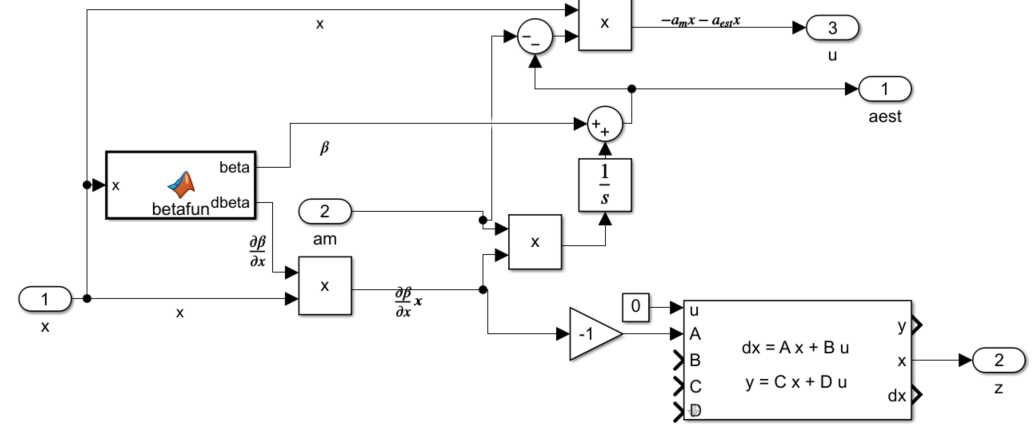
\includegraphics[scale=0.3]{2022-05-19-18-38-24.png} % chktex 8
  \end{figure}
	\end{itemize}
\end{frame}
\begin{frame}
	\frametitle{Simulink - 4}% chktex 8
	\subsection{Controllore MRAC}
	\begin{itemize}
		\item \textbf{MRAC:}
		\begin{figure}
			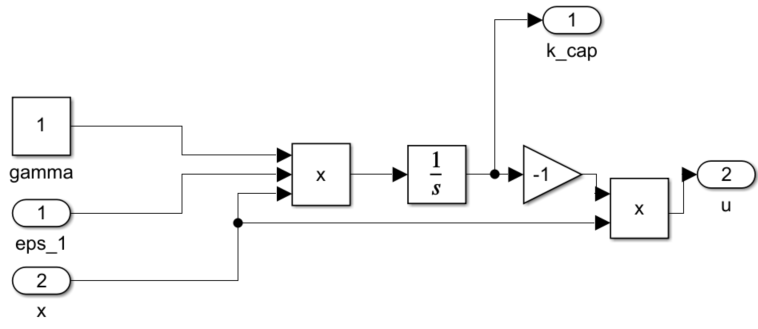
\includegraphics[scale=0.4]{2022-05-19-18-40-36.png}% chktex 8
		\end{figure}
	\end{itemize}
\end{frame}
\begin{frame}
	\frametitle{Simulink - 5}% chktex 8
	\subsection{Sistema complessivo}
\begin{figure}[t]
	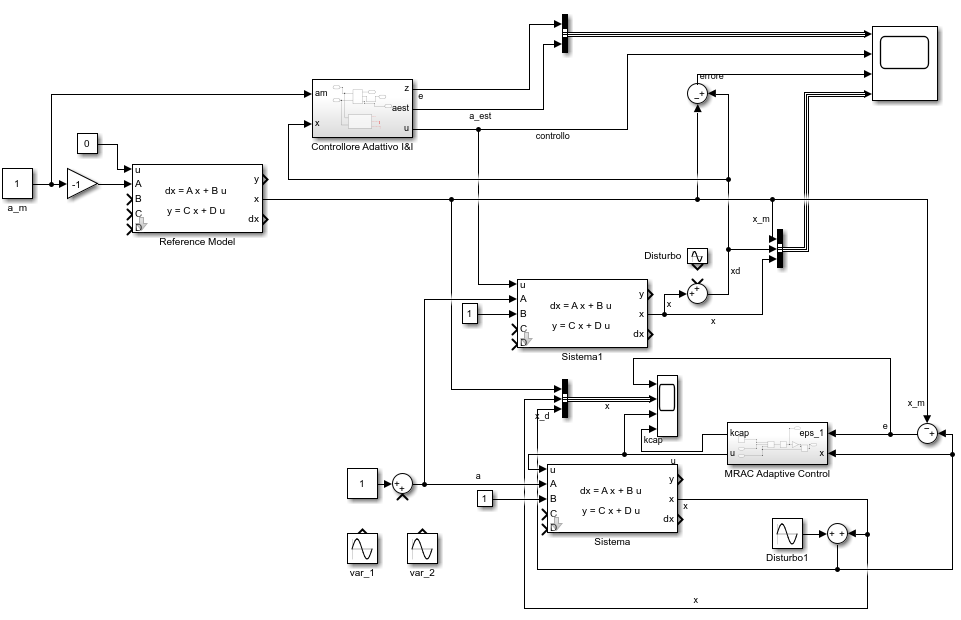
\includegraphics[scale=0.35]{2022-05-20-11-05-07.png}% chktex 8
\end{figure}
\end{frame}
\begin{frame}
	\frametitle{MRAC Parametri stazionari}
	\section{Analisi}
	\subsection{MRAC Parametri stazionari}
	\begin{minipage}[t]{0.45\textwidth}
		\textbf{\(\gamma\) = 1}
		\begin{figure}
			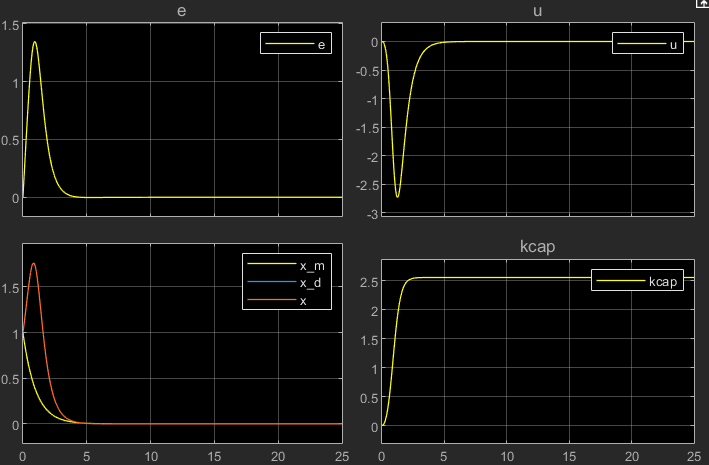
\includegraphics[scale=0.25]{2022-05-20-10-29-19.png} % chktex 8
		\end{figure}
	\end{minipage}
	\begin{minipage}[t]{0.45\textwidth}
		\textbf{\(\gamma\) = 5}
		\begin{figure}
			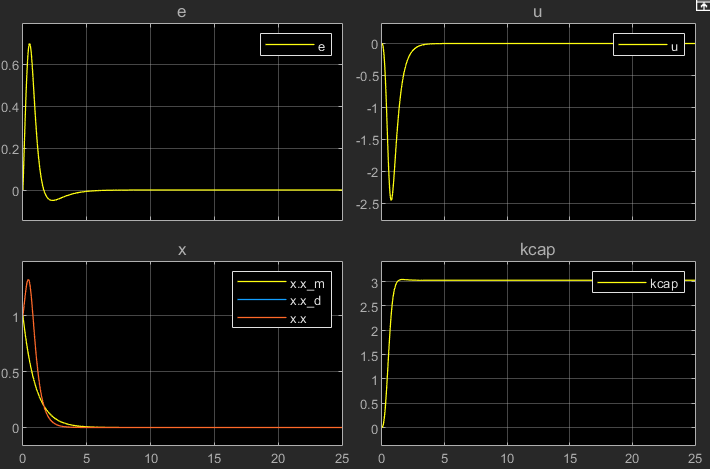
\includegraphics[scale=0.25]{2022-05-20-10-33-35.png} % chktex 8
		\end{figure}
	\end{minipage}
	\vspace{0.1cm}
	\\Al variare del parametro \(\gamma\) del controllore adattativo MRAC si nota che il tempo di convergenza per stimare lo stato rimane invariato a circa 5s. Per valore di \(\gamma\) maggiori, si nota che l'errore presenta una sottoelongazione e la stima di \(k\) una leggera sovraelongazione.
\end{frame}
\begin{frame}
	\frametitle{MRAC Parametri stazionari con rumore}
	\subsection{MRAC Parametri stazionari + rumore}
	\begin{minipage}[t]{0.45\textwidth}
		\textbf{\(\gamma\) = 1}
		\begin{figure}
			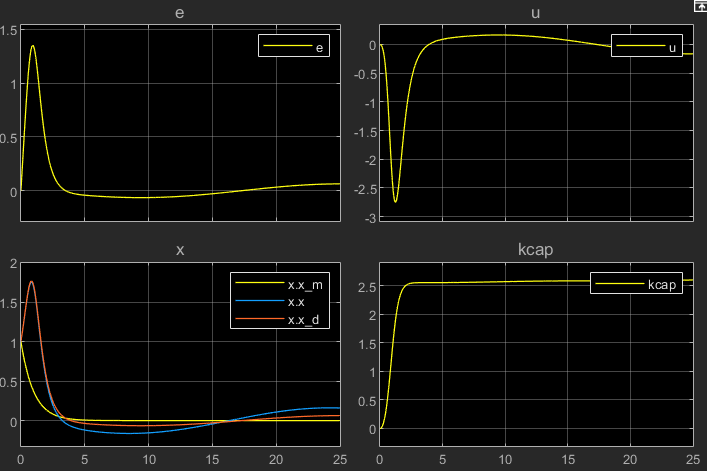
\includegraphics[scale=0.25]{2022-05-20-11-03-08.png} % chktex 8
		\end{figure}
	\end{minipage}
	\begin{minipage}[t]{0.45\textwidth}
		\textbf{\(\gamma\) = 5}
		\begin{figure}
			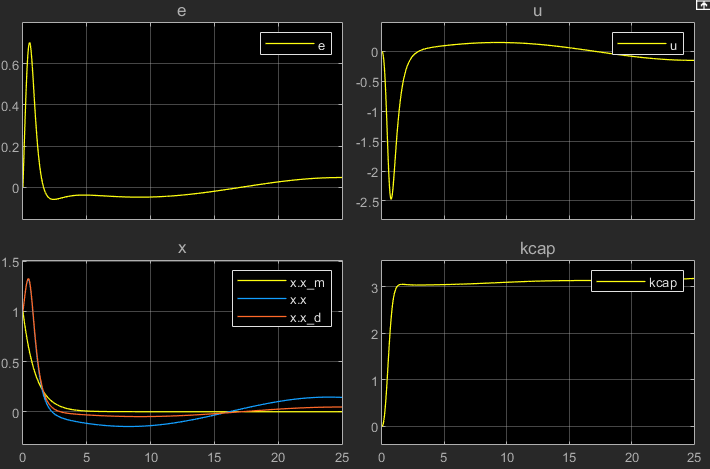
\includegraphics[scale=0.25]{2022-05-20-11-04-01.png} % chktex 8
		\end{figure}
	\end{minipage}
	\vspace{0.1cm}
	L'errore in entrambi i casi rimane limitato, tuttavia a causa del disturbo sinusoidale l'andamento degli stati variano.
\end{frame}
\begin{frame}
	\frametitle{MRAC parametri non stazionari}
	\subsection{MRAC parametri non stazionari}
	\begin{minipage}[t]{0.45\textwidth}
		\textbf{\(\gamma=1\quad a=1+\frac{1}{10}\sin{(10t)}\)}
		\begin{figure}
			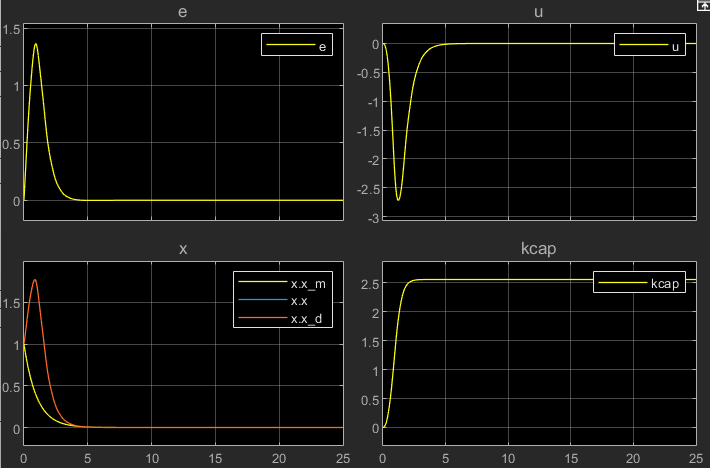
\includegraphics[scale=0.25]{2022-05-20-12-52-05.png} % chktex 8
		\end{figure}
	\end{minipage}
	\begin{minipage}[t]{0.45\textwidth}
		\textbf{\(\gamma=1\quad a=1+10\sin{(\frac{t}{10})}\)}
		\begin{figure}
			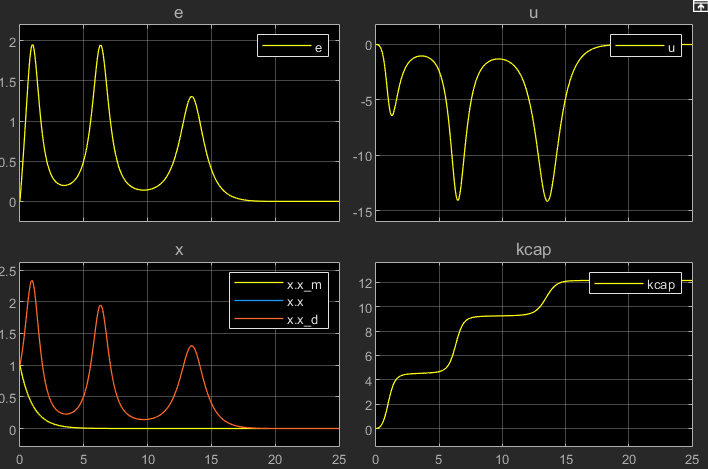
\includegraphics[scale=0.25]{2022-05-20-12-55-10.png} % chktex 8
		\end{figure}
	\end{minipage}
\end{frame}
\begin{frame}
	\frametitle{MRAC parametri non stazionari con rumore}
	\subsection{MRAC parametri non stazionari + rumore}
	\begin{minipage}[t]{0.45\textwidth}
		\textbf{\(\gamma=1\quad a=1+\frac{1}{10}\sin{(10t)}\)}
		\begin{figure}
			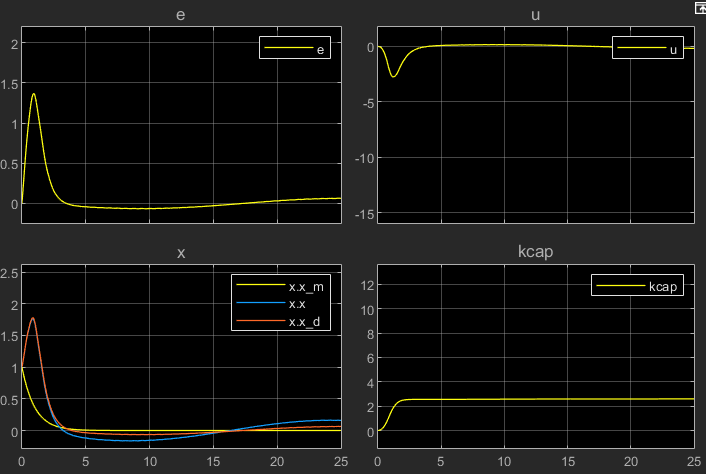
\includegraphics[scale=0.25]{2022-05-20-12-57-45.png} % chktex 8
		\end{figure}
	\end{minipage}
	\begin{minipage}[t]{0.45\textwidth}
		\textbf{\(\gamma=1\quad a=1+10\sin{(\frac{t}{10})}\)}
		\begin{figure}
			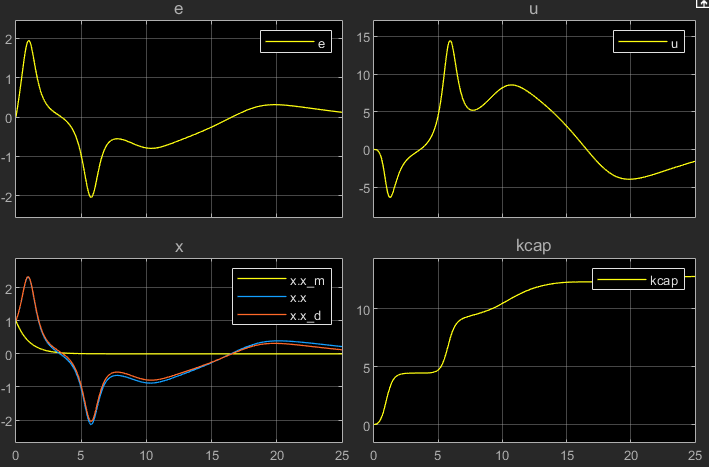
\includegraphics[scale=0.25]{2022-05-20-12-59-29.png} % chktex 8
		\end{figure}
	\end{minipage}
\end{frame}
\begin{frame}
	\frametitle{I\&I parametri stazionari}
	\subsection{I\&I parametri stazionari}

\end{frame}
\begin{frame}
	\frametitle{I\&I parametri stazionari con rumore}
	\subsection{I\&I parametri stazionari + rumore}

\end{frame}
\begin{frame}
	\frametitle{I\&I parametri non stazionari}
	\subsection{I\&I parametri non stazionari}

\end{frame}
\begin{frame}
	\frametitle{I\&I parametri non stazionari con rumore}
	\subsection{I\&I parametri non stazionari + rumore}

\end{frame}
\begin{frame}
	\frametitle{Conclusioni}
	\section{Conclusioni}

\end{frame}
\end{document}